\documentclass[reprint, nofootinbib, nobalancelastpage, 10pt]{revtex4-2}

\usepackage[T2A]{fontenc}			% кодировка
\usepackage[utf8]{inputenc}			% кодировка исходного текста
\usepackage[english,russian]{babel}	% локализация и переносы

\usepackage{amsmath,amsfonts,amssymb,amsthm,mathtools}

\usepackage[usenames]{color}
\usepackage{colortbl}
\usepackage{indentfirst} %Красная строка
\usepackage{hyperref}

\usepackage{booktabs}
\usepackage{graphicx}  % Для вставки рисунков
\graphicspath{{images/}{graphs/}}  % папки с картинками

\renewcommand*{\thefootnote}{\alph{footnote}}

\begin{document}

\title{Изучение рассеяния медленных электронов на атомах (эффект Рамзауэра)}
\author{Илларионов Владислав}
\affiliation{группа Б04-855}

\maketitle


\section*{Введение}

В ходе данной работы исследуется энергетическая зависимость вероятности рассеяния
электронов атомами ксенона, определяются энергии электронов, при которых наблюдается
"просветление" газа, и оценивается размер его внешней электронной оболочки.


\section*{Теоретическая часть}

Качественно результат экспериментов Рамзауэра при энергии электронов порядка десятков
электрон-вольт на аргоне показан на рис.~\ref{img:pic1}

\begin{figure}[h!]
	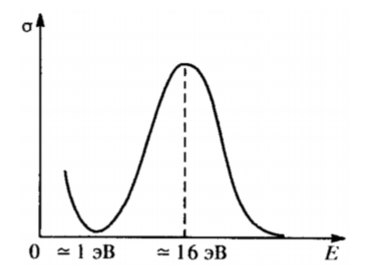
\includegraphics[width = 0.8\linewidth]{pic_1.png}
    \caption{Качественная картина результатов измерения упругого рассеяния электронов в аргоне}
    \label{img:pic1}
\end{figure}

Последующие опыты показали, что это удивительное поведение поперечного сечения свойственно
атомам всех инертных газов.

Для качественного анализа и простых выкладок будем считать, что электрон рассеивается на
одномерной потенциальной яме конечной глубины~(см.~рис.~\ref{img:pic2}).

\begin{figure}[h!]
	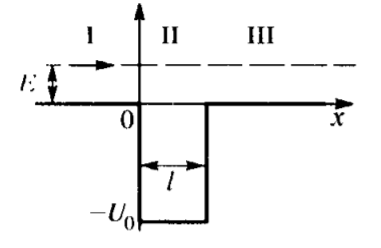
\includegraphics[width = 0.7\linewidth]{pic_2.png}
    \caption{Схематическое изображение прямоугольной ямы, над которой пролетает частица с энергией Е}
    \label{img:pic2}
\end{figure}

Уравнение Шредингера в данном случае имеет вид:

\begin{equation*}
	\psi'' + k^2\psi = 0 \text{, где } k^2 =  
	\begin{cases}
		k^2_1 = \frac{2mE}{\hslash^2} &\text{- в \MakeUppercase{\romannumeral 1}  и \MakeUppercase{\romannumeral 3}}\\
		k^2_2 = \frac{2m(E + U_0)}{\hslash^2} &\text{- в \MakeUppercase{\romannumeral 2}}
	\end{cases}
\end{equation*}

Коэффициент прохождения равен отношению квадратов амплитуд прошедшей и падающей волн и определяется выражением:

\begin{equation*}
	D^{-1} = 1 + \frac{U^2_0}{4E(E + U_0)} \sin^2(k_2l)
\end{equation*}

Коэффициент прохождения частицы над ямой имеет, в зависимости от ее энергии, ряд чередующихся
максимумов и минимумов. В частности, если $k_2l = \pi$, то $\sin (k_2l) = 0$ и коэффициент
прохождения равен единице, электрон беспрепятственно проходит через атом.

Таким образом, коэффициент прохождения электронов максимален при условии:
\begin{equation}
	\label{eq:en}
	k_2l = \sqrt{\frac{2m(E + U_0)}{\hslash^2}}l = n\pi \text{, } n = 1, 2, 3 \ldots
\end{equation}

Получим условия на максимум (\ref{eq:max}) и минимум (\ref{eq:min}) интерференции:

\begin{equation}
    \label{eq:max}
	2l = \frac{h}{\sqrt{2m(E_1 + U_0)}}
\end{equation} 

\begin{equation}
    \label{eq:min}
	2l = \frac{3}{2}\frac{h}{\sqrt{2m(E_2 + U_0)}}
\end{equation}

здесь 2l --- разность хода, $U_0$ - глубина атомного потенциала, $E_1$ и $E_2$ - энергии
электрона, соответствующие этим условиям. Исключая $U_0$, можем найти эффективный размер атома:

\begin{equation}
    \label{eq:l_main}
	l = \frac{h\sqrt{5}}{\sqrt{32m(E_2 - E_1)}}
\end{equation}

Из (\ref{eq:max}) и (\ref{eq:min}) можно также рассчитать эффективную глубину потенциальной ямы атома:

\begin{equation}
    \label{eq:u}
	U_0 = \frac{4}{5}E_2 - \frac{9}{5}E_1
\end{equation}


\section*{Экспериментальная установка}

В данной работе для изучения эффекта Рамзауэра используется тиратрон ТГ3-01/1.3Б,
заполненный инертным газом. Схематическое изображение тиратрона и его конструкция
приведены на рис.~\ref{img:pic4}:

\begin{figure}[h]
	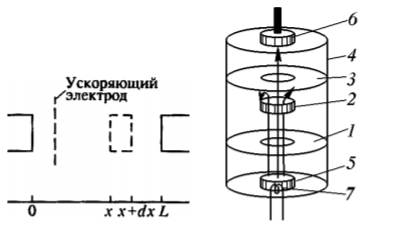
\includegraphics[width = \linewidth]{pic_4.png}
	\caption{Схематическое изображение тиратрона}
	\label{img:pic4}
\end{figure}

Основные элементы тиратрона:

\begin{itemize}
	\item Сетки --- 1, 2, 3
	\item Внешний металлический цилиндр --- 4
	\item Катод --- 5
	\item Анод --- 6
	\item Накапливаемая спираль --- 7
\end{itemize}

Электроны, эмитируемые катодом тиратрона, ускоряются напряжением V, приложеннным между
катодом и ближайшей к нему сеткой. Затем электроны рассеиваются на атомах инертного газа.
Все сетки соединены между собой и имеют одинаковый потенциал(примерно равный потенциалу анода).
Рассеянные электроны отклоняются в сторону и уходят на сетку, а оставшаяся часть электронов
достигает анода и создаёт анодный ток $I_a$.

Принципиальная схема установки для изучения эффекта Рамзауэра приведена на рис.~\ref{img:pic5}.
На лампу Л, расположенную на корпусе БИП подается переменное напряжение частоты 50 Гц,
исследуемый сигнал подается на электронный осциллограф.

\begin{figure}[h!]
	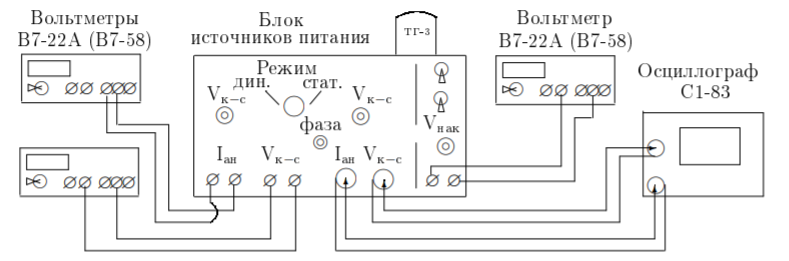
\includegraphics[width = \linewidth]{pic_6.png}
	\caption{Блок-схема экспериментальной установки}
	\label{img:pic5}
\end{figure}

По измеренной ВАХ тиратрона можно определить зависимость вероятности рассеяния электрона
от его энергии из соотношения:

\begin{equation}
	\label{eq:w}
	\omega(V) = -\ln\frac{I_a(V)}{I_0}
\end{equation}

где $I_0$ - ток катода, $I_a$ - анодный ток. Ток анода определяется по показаниям
вольтметра (сопротивление в цепи 100 кОм).


\section*{Методика измерения}

\subsection{Динамический режим}

Для двух значений напряжения накала $V_{\text{н}}$ снимем ВАХ на осциллографе, учитывая его
цену деления. Из полученных из ВАХ значений $U_{min}$ и $U_{max}$ по формулам (\ref{eq:max}),
(\ref{eq:min}) и (\ref{eq:l_main}) определим размер электронной оболочки атома инертного газа,
заполняющего лампу, приняв $U_0 = 2,5$В; по формуле~(\ref{eq:u}) можем также определить значение
эффективной глубины потенциальной ямы атома.

\subsection{Статический режим}

При нескольких разных значениях $V_{\text{н}}$ снимем зависимость $I_a(V_\text{к})$.
Произведем аналогичные расчеты, что и в динамическом режиме.
(Погрешность минимального и максимального значения $I_a$ будем определять из разности
соседних снятых значений ВАХ)

По данным из статического режима по формуле~(\ref{eq:en}) рассчитаем энергии, при которых
должны появляться максимумы в коэффициенте прохождения электронов для $n$ = 2, 3.

На основе формулы~(\ref{eq:w}) найдем зависимость вероятности рассеяния электронов
(с точностью до константы) от энергии и построим соответствующий график.


\section*{Обработка данных}

По данным динамического режима рассчитаем приблизительный радиус электронной оболочки атома
газа по формулам и глубину его потенциальной ямы. Результаты вычислений занесем в таблицу~\ref{tab:1}.

В статическом режиме снимем зависимость $I_a(V_\text{к})$ и построим графики для трех
значений $V_{\text{н}}$~(см.~рис.~\ref{graph:plot1})

\begin{figure}[h!]
	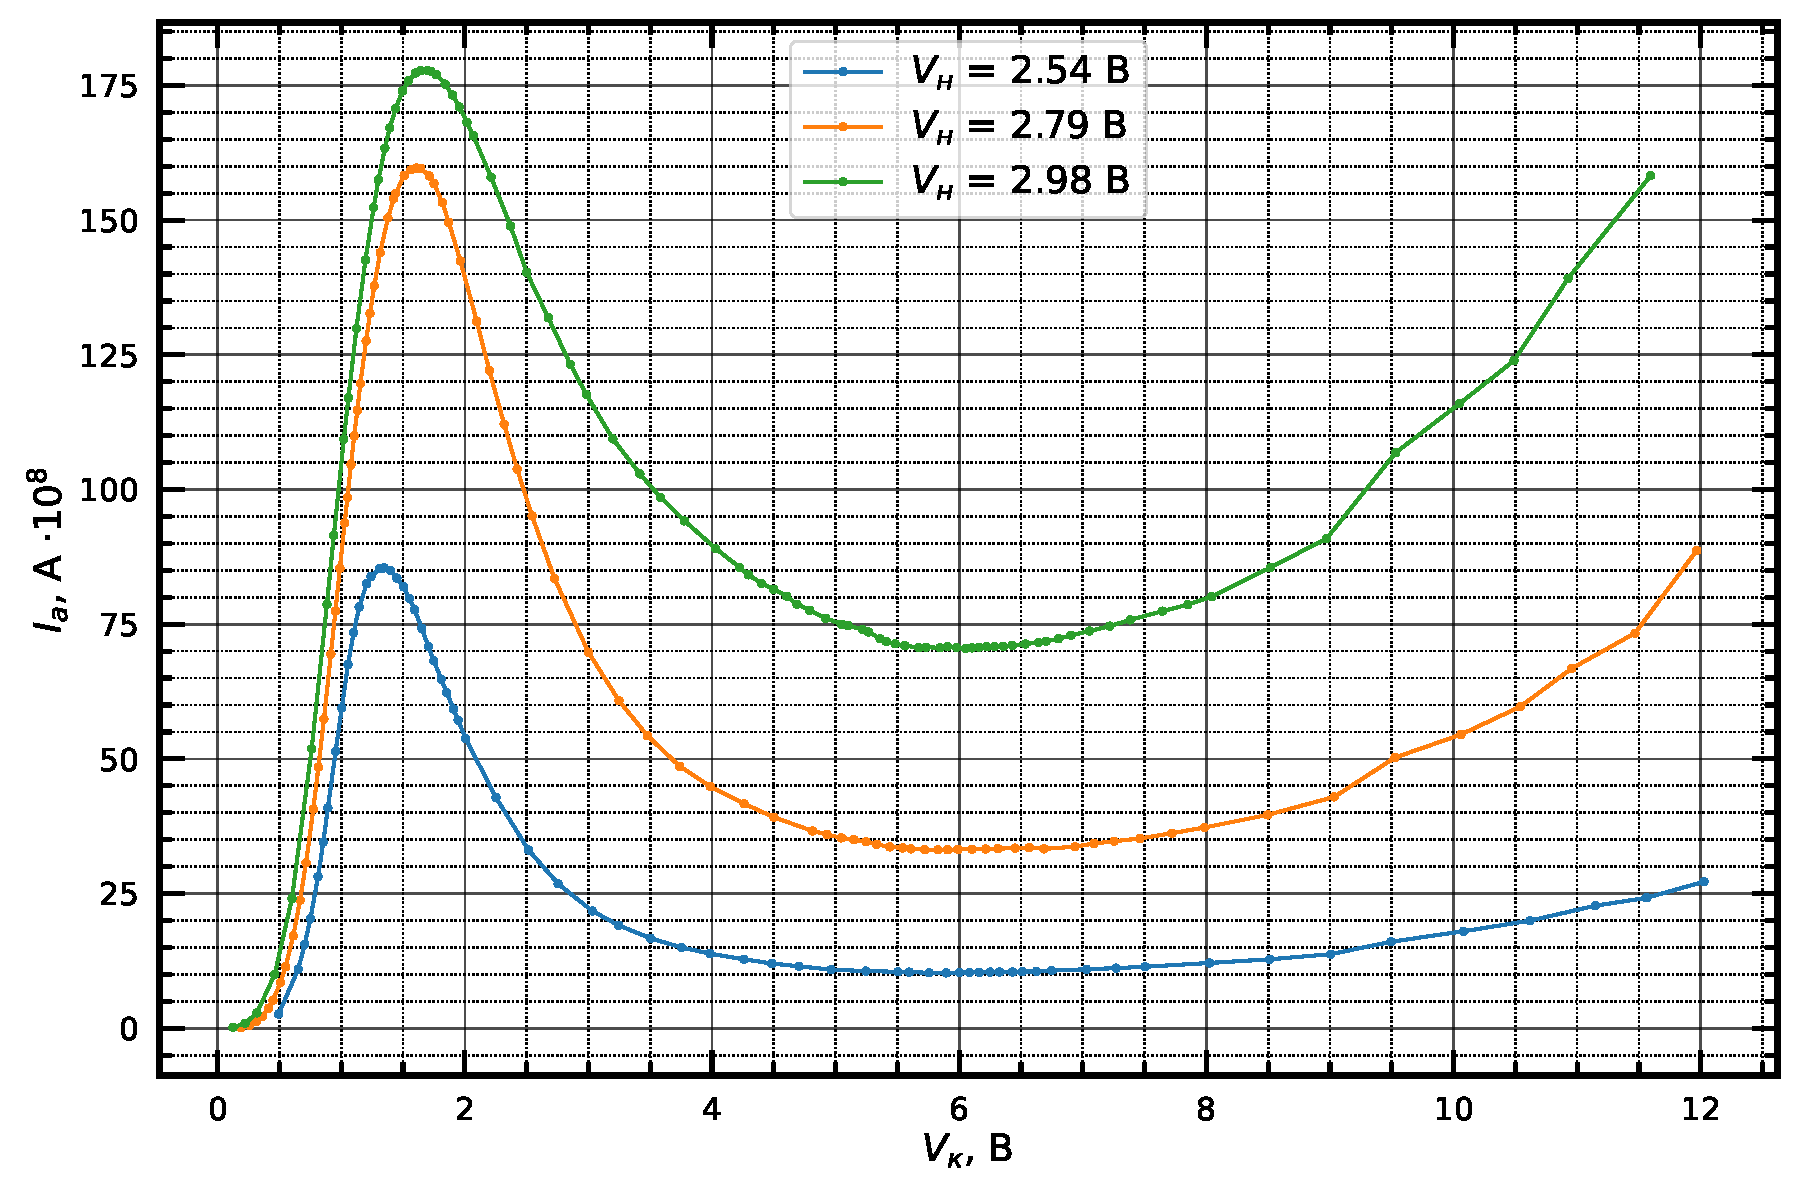
\includegraphics[width = \linewidth]{vah.pdf}
	\caption{График зависимости анодного тока от ускоряющего напряжения}
	\label{graph:plot1}
\end{figure}

По данным статического режима проведем аналогичные динамическому режиму вычисления и занесем
результаты в таблицу~\ref{tab:2}

По данным из статического режима по формуле~(\ref{eq:en}) рассчитаем энергии, при которых
должны появляться максимумы в коэффициенте прохождения электронов для $n$ = 2, 3.
Результаты занесем в таблицу~\ref{tab:3}.

Согласно формуле~(\ref{eq:w}) найдем зависимость вероятности рассеяния электронов от энергии электрона
(с точностью до константы) и построим соответствующий график~(см.~рис.~\ref{graph:plot2})

\begin{figure}[h!]
	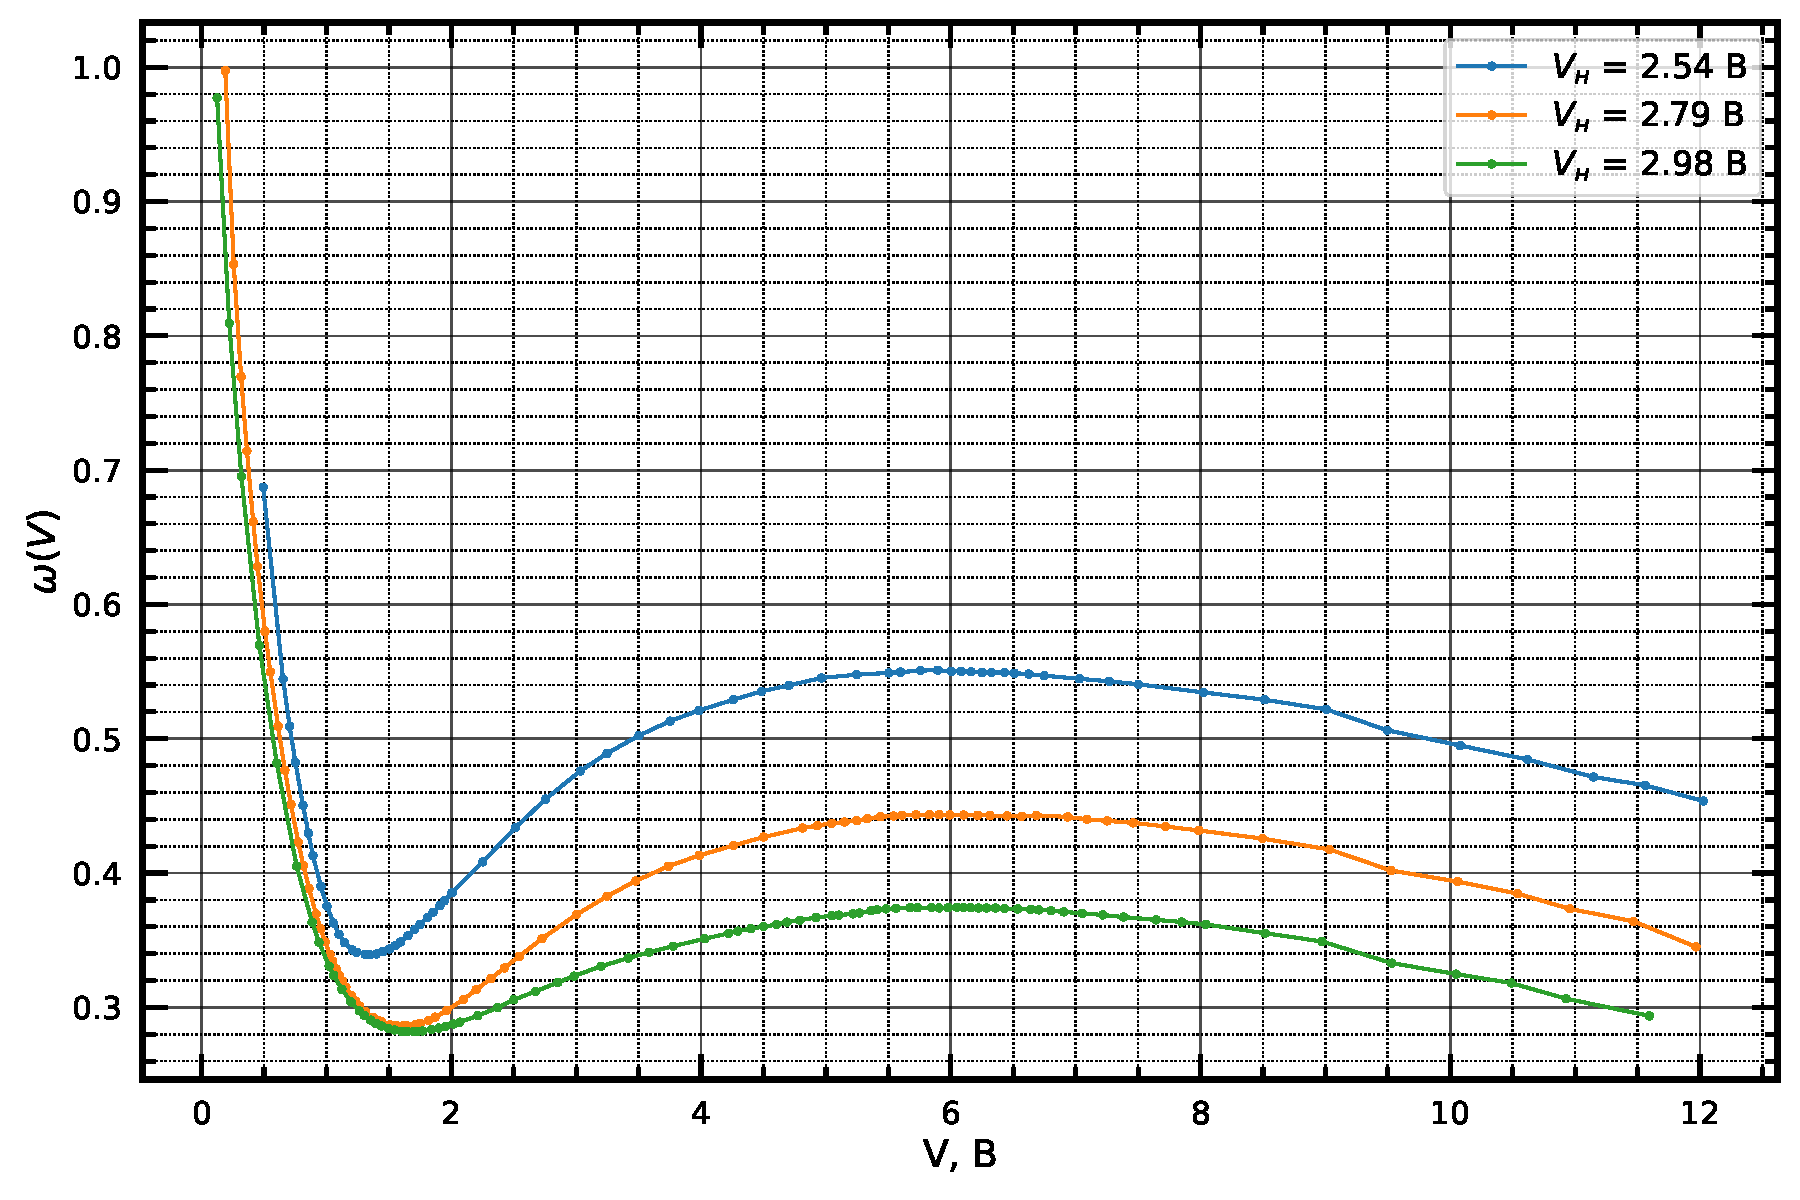
\includegraphics[width = \linewidth]{w.pdf}
	\caption{График зависимости вероятности рассеяния электронов от ускоряющего напряжения с точностью до константы}
	\label{graph:plot2}
\end{figure}

\newpage

\section*{Вывод}

В ходе данной работы был изучен эффект Рамзауэра рассеяния медленных электронов на атомах ксенона.
На основе формул, полученных при рассмотрении интерференции электронных волн де Бройля в атоме,
были вычислены диаметр электронной оболочки атома и глубина его потенциальной ямы в динамическом и
статическом методах измерения.

Погрешности значений $l$, полученных в динамическом методе~(табл.~\ref{tab:1}), обусловлены
ценой деления осциллографа 1 В/дел. Неточность в определении $U_0$ в динамическом режиме
может быть связана с неправильным определением минимума анодного тока по осциллографу, т.к.
зависимость была пологая.

Значения $l$, полученные в статическом методе~(табл.~\ref{tab:2}) намного точнее и близки
к диаметру Ван дер Ваальса ксенона (2.9\AA)

Значения $U_0$ полученные в статическом методе, не совпадают со значением, данным в учебнике.
Неточность определения $U_0$ может быть связана с грубостью модели одномерной потенциальной
ямы.

\newpage
\appendix

\onecolumngrid
\section{Таблицы}


\begin{table}[h!]
	\caption{Динамический режим}
	\label{tab:1}
	\begin{tabular}{|p{2cm}|p{2cm}|p{2cm}|p{2cm}|p{2cm}|p{2cm}|p{2cm}|}
		\hline
		$V_{\text{н}}$, В & $E_{max}$, эВ & $E_{min}$, эВ & $l$(\ref{eq:max}), \AA{} & $l$(\ref{eq:min}), \AA{} & $l$(\ref{eq:l_main}), \AA{} & $U_0$, эВ \\ \hline
		2,793 & 2,6 $\pm$  0,3 & 5,6 $\pm$ 0,3 & 2,72 $\pm$ 0,15 & 3,23 $\pm$ 0,08 & 3,96 $\pm$ 0,26 & -0,2 $\pm$ 0,6  \\ \hline
		2,516 & 3 $\pm$ 0,3   & 5,8 $\pm$ 0,3 & 2,62 $\pm$ 0,12 & 3,19 $\pm$ 0,08 & 4,1 $\pm$ 0,3   & -0,76 $\pm$ 0,6 \\ \hline
	\end{tabular}
\end{table}

\begin{table}[h!]
	\caption{Статический режим}
	\label{tab:2}
	\begin{tabular}{|p{2cm}|p{2cm}|p{2cm}|p{2cm}|p{2cm}|p{2cm}|p{2cm}|}
		\hline
		$V_{\text{н}}$, В     & $E_{max}$,  эВ        & $E_{min}$,  эВ        &  $l$(\ref{eq:max}), \AA{} & $l$(\ref{eq:min}), \AA{} & $l$(\ref{eq:l_main}), \AA{}        &  $U_0$, эВ         \\ \hline
		2,540 & 1,33 $\pm$  0,04 & 5,83 $\pm$ 0,14 & 3,14 $\pm$ 0,04 & 3,19 $\pm$ 0,04 & 3,23 $\pm$ 0,05 & 2,27 $\pm$ 0,13  \\ \hline
		2,795 & 1,63 $\pm$ 0,03   & 5,87 $\pm$ 0,08 & 3,02 $\pm$ 0,03 & 3,18 $\pm$ 0,02 & 3,33 $\pm$ 0,03   & 1,77 $\pm$ 0,09 \\ \hline
		2,983 & 1,67 $\pm$ 0,05   & 6,08 $\pm$ 0,05 & 3,00 $\pm$ 0,05 & 3,14 $\pm$ 0,01 & 3,27 $\pm$ 0,03   & 1,85 $\pm$ 0,11 \\ \hline
	\end{tabular}
\end{table}

\begin{table}[h!]
	\caption{Энергии для 2 и 3 максимума коэффициента прохождения}
	\label{tab:3}
	\begin{tabular}{|p{2cm}|p{2cm}|p{2cm}|}
		\hline
		$V_{\text{н}}$,В & $E_2$, эВ & $E_3$, эВ    \\ \hline
		2,540 & 15,15 $\pm$ 0,48 & 33,14 $\pm$ 1,04 \\ \hline
		2,795 & 14,33 $\pm$ 0,29 & 31,29 $\pm$ 0,62 \\ \hline
		2,983 & 14,86 $\pm$ 0,26 & 32,48 $\pm$ 0,56 \\ \hline
	\end{tabular}
\end{table}

\section{ВАХ в динамическом режиме}

\twocolumngrid

\begin{figure}[h!]
	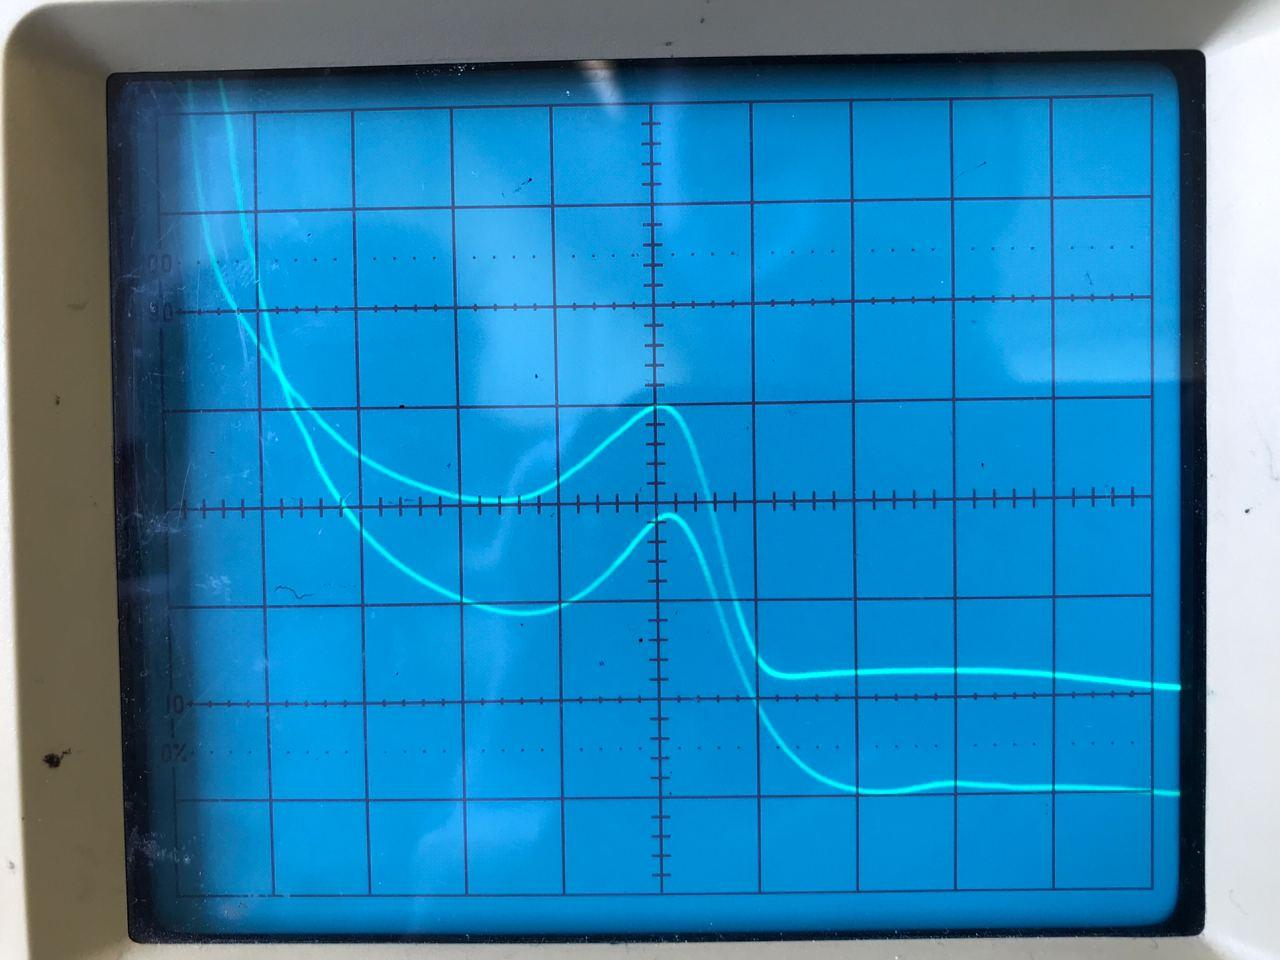
\includegraphics[width = \linewidth]{vah1.jpg}
	\caption{ВАХ в динамическом режиме для $V_{\text{н}} = 2.793 B$}
	\label{graph:dinvah1}
\end{figure}

\begin{figure}[h!]
	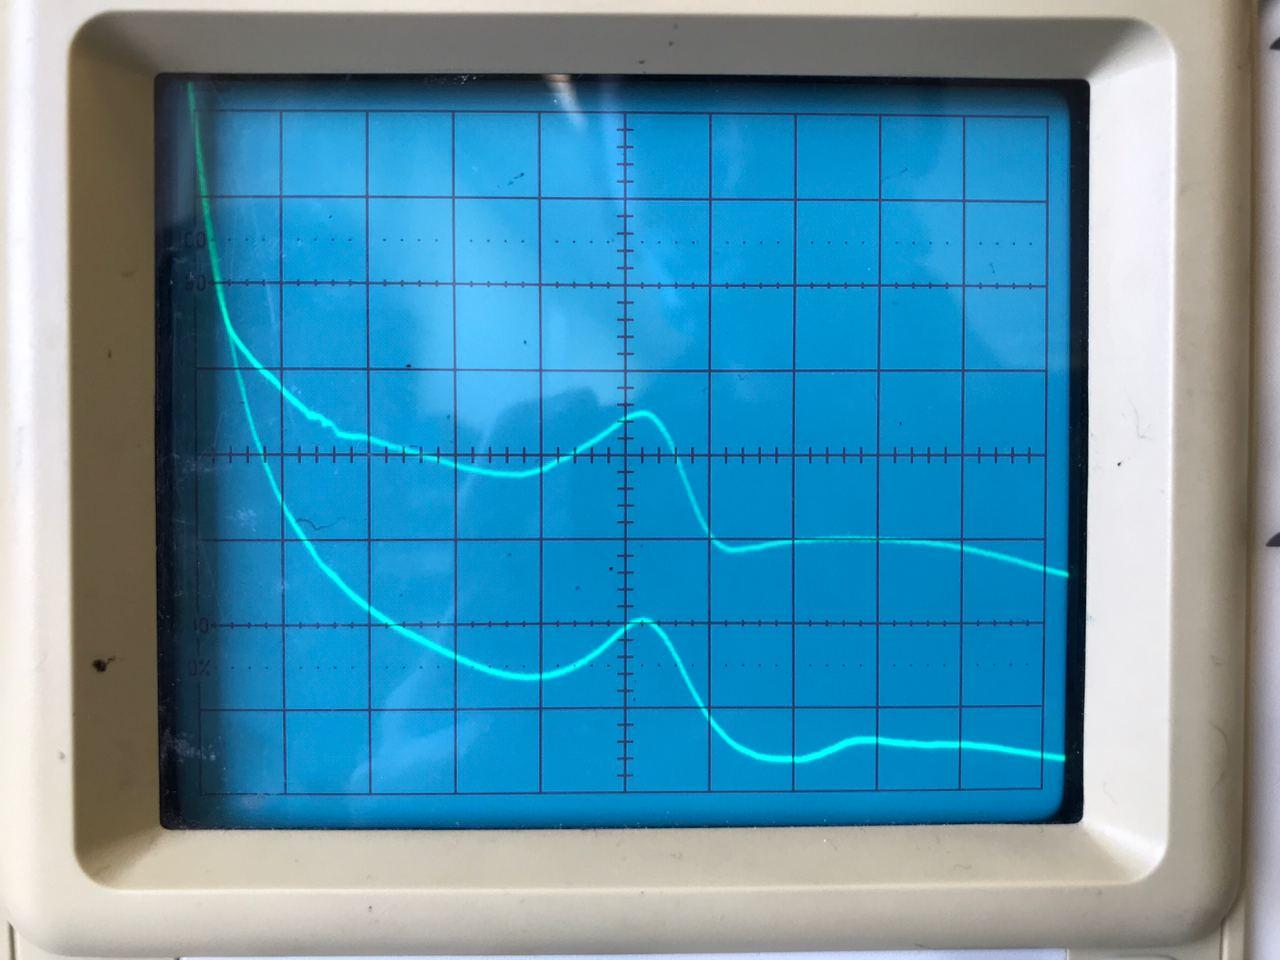
\includegraphics[width = \linewidth]{vah2.jpg}
	\caption{ВАХ в динамическом режиме для $V_{\text{н}} = 2.516 B$}
	\label{graph:dinvah2}
\end{figure}


\end{document}